\documentclass[10pt,journal,letterpaper]{IEEEtran}
\usepackage[letterpaper, left=0.65in, right=0.65in, bottom=0.7in, top=0.7in]{geometry}
\usepackage{tikz}
\usetikzlibrary{arrows.meta}
\usepackage{mathptmx}
\usepackage{lipsum}
\usepackage{cite}
\usepackage{amsmath,amssymb,amsfonts}
\usepackage{algorithmic}
\usepackage{graphicx}
\usepackage{textcomp}
\usepackage{xcolor}
\usepackage{nicefrac}
\usepackage{type1cm}
\usepackage{lettrine}
\usepackage{makecell}
\usepackage{fancyhdr}
\usepackage[none]{hyphenat}
\usepackage{float}
\usepackage[draft]{hyperref}
\usepackage{multirow}
\usepackage{import}
\usepackage{xifthen}
\usepackage{pdfpages}
\usepackage[siunitx]{circuitikz}
\usepackage{siunitx}
\usepackage{transparent}
\usepackage{microtype}

\graphicspath{ {./figures/} }

\newcommand{\incfig}[1]{%
	\centering
    \import{./figures/}{#1.pdf_tex}
}
    
\pagestyle{fancy}
\fancyhf{}
\renewcommand{\headrulewidth}{0pt}
\rhead{\thepage}
\lhead{Lab Final}

\setlength{\columnsep}{0.2in}
\setlength{\columnwidth}{3.5in}

\sisetup{per-mode = symbol,
	inter-unit-product = \ensuremath{{}\cdot{}}
}

\newcommand{\todo}{\textcolor{red}{???}}

\newcommand{\co}{CO\textsubscript{2}}

\begin{document}
\title{Determination of Pressure Inside of a Beverage Can}

\author{\IEEEauthorblockN{\huge{Hornilla, Joshua \\ Hutt, Kateland \\ Latzko, Alexander \\ Sukhadia, Kenni \\}}
\IEEEauthorblockA{
Group 50 \quad April 22, 2022}
}

\maketitle
\thispagestyle{empty}

\begin{abstract}
This experiment uses knowledge of the two-dimensional principal stress state to determine the internal pressure in an unopened soda can.
Thin-walled pressure vessel theory is used in conjunction with theories on principal stresses to report the internal can pressure.
This result is compared to another method based upon the ideal gas law.
The hoop stress in the can is 78.11 $\pm$ 1.128 MPa and the longitudinal stress is 46.27 $\pm$ 0.677 MPa.
The internal pressure reported by the mechanics of materials approach is 252 $\pm$ 43.4 kPa.
The internal pressure reported by the ideal gas law method is 258 $\pm$ 57.2 kPa.
\end{abstract}

\begin{IEEEkeywords}
plane stress, principal stresses, strain gauge rosette, thin-walled pressure vessel
\end{IEEEkeywords}

\section{Introduction}
\IEEEPARstart{C}{ylindrical} pressure vessels are an effective way to store gasses or liquids which must be kept at high pressures.
As such, knowing the operating and current pressures in these vessels is imperative to ensuring user safety; catastrophic failures in these vessels can sometimes be fatal.
The stresses in the walls of these vessels can be used to determine the overall pressure within the vessel.
This study seeks to determine the pressure in a sealed soda can.

The can is a thin-walled pressure vessel.
The diameter of the can is much greater than its wall thickness, leading to the assumption that there is no stress in the direction of the thickness of the can, so the stresses in the vessel wall can be analyzed as a two-dimensional stress state, or the plane stress condition.

To analyze this stress state, strain gauges can be affixed in a 0-45-\ang{90} rosette on the side of the can to record the strains on the walls.
Using multiple strain gauges allows an experimenter to determine the complete strain state, including the shear strain.
As the strain gauge is a transducer, the strains are recorded as a voltage difference, $\Delta V_{g}$, and are calculated according to \eqref{eq:strain}, where $V_s$ is the excitation voltage for the circuit, $G_f$ is the gauge factor of the strain gauge, given by the manufacturer, and $A$ is the gain of the amplifier \cite{b1}.
\begin{equation}
\label{eq:strain}
\varepsilon=\frac{4\Delta V_g}{A V_s G_f}
\end{equation}

These strain gauges work in conjunction with a quarter Wheatstone bridge circuit to record meaningful voltage differences (Fig. \ref{fig:Wheatstone}).
The strain gauge acts as a variable resistor.
The change in voltage across the bridge as the strain gauge moves and varies its resistance is the voltage used to compute strain in \eqref{eq:strain}.
Each gauge in the strain gauge rosette has its own individual Wheatstone bridge circuit fed by an excitation voltage.

\begin{figure}[H]
\centering
\begin{circuitikz}[american voltages, scale=1.75]
\ctikzset{label/align = straight}
  \draw (0,0) to[V, invert, l_=$V_s$] (0,2) -- (2,2)
  to[R, l_=$R_4$,*-*] (1,1)
  to[R, l_=$R_3$, *-*] (2,0) -- (0,0);

 \draw (2,2) to[R=$R_1$, *-*] (3,1) to (2.9,0.9) to (3.3,0.9) to[european resistor=$R_2$] (3.3,0.1) to (2.1,0.1) to (2,0);
 \draw (1,1) to[rmeter, t=$V_g$] (3,1);
 \draw (3.3,0.5) node[left=0.8em,align=left] {Strain\\gauge};
 \end{circuitikz}
\caption{A simple quarter Wheatstone bridge circuit. Ideally, all resistances are equal.}
\label{fig:Wheatstone}
\end{figure}

In plane strain, the shear strain $\gamma_{xy}$ can be computed using the \ang{45} strain gauge value according to \eqref{eq:strainThet}, where $\varepsilon_x$ and $\varepsilon_y$ are the strains from the \ang{0} and \ang{90} strain gauges, respectively, and $\theta$ is \ang{45} for this rosette \cite{b5}.
\begin{equation}
\label{eq:strainThet}
\varepsilon_\theta=\frac{\varepsilon_x+\varepsilon_y}{2}-\frac{\varepsilon_x-\varepsilon_y}{2}\cos(2\theta)+\gamma_{xy}\sin(2\theta)
\end{equation}

While the experimenter should attempt to align the strain gauge rosette along the principal axes, along the can's central axis and along its circumference, the true principal strain should be found according to \eqref{eq:princStrain}, where $\varepsilon_{1,2}$ are the principal strains for the plane strain condition.
This is based upon the concepts of Mohr’s circle, a way to identify principal stresses and strains in a material geometrically.
\begin{equation}
\label{eq:princStrain}
\varepsilon_{1,2}=\frac{\varepsilon_x+\varepsilon_y}{2} \pm \sqrt{\left(\frac{\varepsilon_x-\varepsilon_y}{2}\right)^2+\left(\frac{\gamma_{xy}}{2}\right)^2}
\end{equation}

Knowing the principal strains, the principal stresses in the vessel can be computed.
These principal stresses in the wall arise from the internal pressure pushing on the can wall, so knowing the principal stresses in the wall allows the pressure within the can to be calculated.
In 2D strain, Hooke's law relating stress to strain is given directionally as \eqref{eq:sigma1} and \eqref{eq:sigma2}, where $\sigma_{1}$ and $\sigma_{2}$ are the principal stress on the wall, $E$ is the modulus of elasticity of the can material, which is aluminum 3004-H19 \cite{b2}, $\nu$ is Poisson’s ratio of the can material, and $\varepsilon_{1}$ and $\varepsilon_{2}$ are the principal strains, found by using \eqref{eq:princStrain} with the recorded strains \cite{b1}.
\begin{subequations}
\label{eq:sigmas}
\begin{align}
\sigma_1&=\frac{E}{1-\nu^2}\left(\varepsilon_1+\nu\varepsilon_2\right) \label{eq:sigma1} \\
\sigma_2&=\frac{E}{1-\nu^2}\left(\varepsilon_2+\nu\varepsilon_1\right) \label{eq:sigma2}
\end{align}
\end{subequations}

For thin-walled pressure vessels, the 2D stress state is described by the longitudinal stress, along the vessel's central axis, and hoop stress, along its circumference, which can be computed with the principal strains above.
The free-body diagram (Fig. \ref{fig:PVessel}) can be a helpful tool in relating these stresses to the can's internal pressure \cite{b1}.

\begin{figure}[H]
\centering
\includegraphics[width=3in]{PVessel}
\caption{Free-body diagram of the pressures acting on the pressure vessel internally.}
\label{fig:PVessel}
\end{figure}

The force balance for this diagram is \eqref{eq:vesselForce},
\begin{equation}
\label{eq:vesselForce}
(2rL)P=(2Lt)\sigma_H
\end{equation}
as pressure $P$ acts on the can inner surface area, $2rL$, and is resisted by the circumferential hoop stress $\sigma_H$ acting on wall area $2Lt$.
The expression \eqref{eq:vesselForce} can be solved for the hoop stress $\sigma_H$ using \eqref{eq:hoopStress}.
\begin{equation}
\label{eq:hoopStress}
\sigma_H=\frac{Pr}{t}
\end{equation}

This hoop stress is related to its orthogonal longitudinal stress $\sigma_L$ with \eqref{eq:longStress}, known from thin-walled pressure vessel theory \cite{b1}.
\begin{equation}
\label{eq:longStress}
\sigma_L=\frac{1}{2}\sigma_H
\end{equation}

These hoop and longitudinal stresses are assumed to be the principal stresses $\sigma_1$ and $\sigma_2$.
Thus, the relationships from \eqref{eq:hoopStress} and \eqref{eq:sigmas} can be rearranged to yield \eqref{eq:princStrainFin}, a functional relationship between principal strain and internal pressure \cite{b1}.
\begin{equation}
\label{eq:princStrainFin}
\varepsilon_1=\frac{Pr}{2Et}(2-\nu)
\end{equation}

Soda is carbonated by being bottled with carbon dioxide (\co) under high pressure \cite{b9}.
Because the soda itself is negligibly compressible in comparison to the gaseous \co , the pressure can be assumed to be caused only by the \co .
Therefore, the pressure in the vessel can be determined by measuring the \co\ that escapes during depressurization.
The ideal gas law, \eqref{eq:IGL}, can be used to estimate this pressure.
\begin{equation}
\label{eq:IGL}
PV=nRT
\end{equation}
where $P$ is pressure, $V$ is volume, $n$ is the number of moles, $R$ is the gas constant, and $T$ is the temperature.
Solving for pressure gives \eqref{eq:PIGL}.
\begin{equation}
\label{eq:PIGL}
P = \frac{nRT}{V}
\end{equation}

By weighing the can before and after depressurization, the amount of escaped \co, $n$, can be calculated using \eqref{eq:moles}, where $W_{ci}$ is the initial weight of the can, $W_{cf}$ is the weight of the can after depressurization, and $M$ is the molar mass of \co.
\begin{equation}
\label{eq:moles}
n=\frac{W_{ci}-W_{cf}}{M}
\end{equation}

The volume occupied by the \co\ can be calculated by measuring the weight of water required to fill that space using \eqref{eq:vol}, where $W_{wi}$ is the initial weight of the water container, $W_{cf}$ is the final weight of the water container, and $\rho$ is the density of water.
\begin{equation}
\label{eq:vol}
V=\frac{W_{wi}-W_{wf}}{\rho}
\end{equation}

Assuming the can is left in a room for a significant amount of time, the temperature of that room can be measured and will be accurate for the can's contents \cite{b9}.

\section{Procedure}

\subsection{Supplies Required}

The supplies needed for this experiment include a data acquisition system (DAQ) and a soda can.
A strain gauge rosette and cyanoacrylate glue is also required.
A container with an arbitrary amount of water, packing tape, painter's tape, fine sandpaper, and methanol for cleaning the can surface are needed.
A micrometer is needed to measure the diameter of the can and the thickness its material.
A scale is needed to measure the weight of the can and the container of water.
A thermometer is needed to measure the temperature of the room.
Three amplifiers, nine known resistors with the same resistance as the strain gauge rosette, a breadboard, various wires, solder, a soldering iron, and an external power supply are needed to make the Wheatstone bridge circuits.
A LabVIEW virtual instrument (VI) is used to record the data.
Table \ref{tab:mats} shows the details of the equipment used in this specific lab.
\begin{table}[H]
\renewcommand\arraystretch{1.25}
\centering
\caption{Specific Equipment Used in this Lab}
\begin{tabular}{cc}
\hline \hline
Equipment & Specification \\
\hline
DAQ & Out of the Box SADI \\
350 \unit{\ohm} strain gauge rosette & Omega SGD-3/350-RYT23 \\
3 Amplifiers & Texas Instruments THS4522 \\
9 Resistors & 350 \unit{\ohm} \\
\hline \hline
\end{tabular}
\label{tab:mats}
\end{table}

\subsection{Instrumenting the Soda Can}

The can must first be outfitted with the strain gauge rosette.
First, the decorative wrapping on the beverage can is scrubbed off with fine sandpaper so that this wrapping does not affect the strain response of the can.
Once the surface is properly cleaned using methanol, painter's tape is used to create an approximately \ang{90} L-shaped guideline towards the outer left and bottom edges of the cleaned surface for strain gauge placement.

To place the strain gauge rosette, clear packing tape is placed over the top of the rosette, opposite the side that will contact the surface of the can.
The tacky side of the taped strain rosette is then gently laid onto the can surface, such that the \ang{0} and \ang{90} strain gauges are aligned with the taped guidelines.
When the placement of the strain rosette is properly aligned, part of the taped side is lifted, and glue is applied to the can.
The strain gauge rosette is replaced over top of the glue and is left to cure. 

\subsection{Wheatstone Bridge}

Each strain gauge works as a variable resistor in a Wheatstone bridge, where the voltage difference across the bridge is recorded for the strain (Fig. \ref{fig:Wheatstone}).
Three Wheatstone bridge configurations are wired onto a simple breadboard.
Each bridge also makes use of an amplifier, as the voltages passing through the circuit are expected to be very small.
An excitation voltage $V_s$ of 3.3 V is wired so as to pass across each bridge from the external power supply due to the DAQ being limited to 30 mA \cite{b10}.
This excitation voltage $V_s$ and the amplified bridge voltage $V_{amp}$ for each of the three bridges is recorded with the DAQ.

\subsection{Data Acquisition}

The DAQ which records the voltage difference is fed into the LabVIEW VI.
This VI reads the $V_{amp}$ for each bridge as $V_{amp_x}$ for the \ang{0} gauge, $V_{amp_\theta}$  for the \ang{45} gauge, and $V_{amp_y}$ for the \ang{90} gauge.
These are observed with a $\pm$5.12 V gain window.

First, the VI is run on the undisturbed instrumented soda can and voltage data is collected for taring purposes.
The $V_{amp}$ values are then tared in order to eliminate bias error.
The $V_{amp}$ values for each bridge and the excitation voltage $V_s$ are recorded by the VI before, during, and after the can is opened. 

\subsection{Ideal Gas Law Pressure Determination Method}

A secondary method based upon the ideal gas law is also used.
For this method, the temperature of the room is measured and the can is allowed to reach thermodynamic equilibrium with the room.
The unopened, instrumented can is weighed on a scale, and its initial weight is recorded.
After the can is opened, the instrumented can is weighed again and its final weight is recorded.
Next, a bottle filled with an arbitrary amount of water is weighed on the scale.
Water is poured from the bottle into the open can until the headspace between the soda and the top of the can is filled.
The bottle is weighed again \cite{b9}.

\section{Results}

The beverage can that the group originally instrumented during this lab suffered a short in the circuit.
Thus, all $V_{amp}$ readings recorded the excitation voltage rather than the voltage differences in the strain rosette.
As such, the data used for the instrumented can is supplied by Dr. Ridgeway, and collected by a different student group from the Fall 2021 semester of EML3301C.
The type of beverage that this data represents was not reported.
The ideal gas law method data was collected in lab by the authors.

\subsection{Can Properties}

The can properties measured in lab for use in the ideal gas law method are presented in Table \ref{tab:IGLProp}.
All weights were measured by the same digital scale.
The ambient temperature of the room was measured by a mercury thermometer and the can was left unrefrigerated in the room long enough to reach ambient temperature.
\begin{table}[H]
\renewcommand\arraystretch{1.25}
\centering
\caption{Can Properties for Ideal Gas Law Method}
\begin{tabular}{cc}
\hline \hline
Property & Value \\
\hline
Initial Can Weight & 406.8 $\pm$ 0.1 g \\
Final Can Weight & 406.2 $\pm$ 0.1 g \\
Initial Water Weight & 152.0 $\pm$ 0.1 g \\
Final Water Weight & 141.1 $\pm$ 0.1 g \\
Ambient Temperature & 22.78 $\pm$ 0.28\unit{\celsius} \\
\hline \hline
\end{tabular}
\label{tab:IGLProp}
\end{table}

The can properties measured by the Fall 2021 student group and used in this report for the mechanics of materials method are presented in Table \ref{tab:MoMProp}.
These values were measured four times with a micrometer and a 95\% confidence interval was calculated for the uncertainties.
\begin{table}[H]
\renewcommand\arraystretch{1.25}
\centering
\caption{Can Properties for Mechanics of Materials Method}
\begin{tabular}{cc}
\hline \hline
Property & Value (mm) \\
\hline
Can Thickness & 0.091 $\pm$ 0.016 \\
Can Diameter & 66.63 $\pm$ 0.89 \\
\hline \hline
\end{tabular}
\label{tab:MoMProp}
\end{table}

\subsection{Recorded Voltages}

By examining the data from Fall 2021, it is determined that four voltages were continuously recorded before, during, and after the can was opened.
The data is assumed to have been taken at a frequency of 0.5 kHz.
This assumption does not impact the conclusions drawn from the data, as only the steady state values before and after the can was opened are considered.
The three amplified voltages from the strain rosette show the can being opened just after one second into data collection (Fig. \ref{fig:VampTime}).
The steady state data before and after can opening are isolated and individually reported.
The mean and standard deviation for the three amplified voltages before and after can opening and the excitation voltage, $V_s$, are presented in Table \ref{tab:RecV}.
\begin{figure}[H]
\def\svgwidth{2.75in}
\incfig{VampTime}
\caption{Captured voltages versus time.}
\label{fig:VampTime}
\end{figure}

\begin{table}[H]
\renewcommand\arraystretch{1.25}
\centering
\caption{Recorded Voltages}
\begin{tabular}{ccc}
\hline \hline
Voltage & Initial (V) & Final (V) \\
\hline
$V_{amp_x}$ & $-$0.1389 $\pm$ 0.00056 & $-$0.2367 $\pm$ 0.0011 \\
$V_{amp_\theta}$ & 0.0674 $\pm$ 0.00039 & $-$0.0253 $\pm$ 0.00027 \\
$V_{amp_y}$ & $-$0.1064 $\pm$ 0.00052 & $-$0.1398 $\pm$ 0.00055 \\
$V_{s}$ & \multicolumn{2}{c}{3.349 $\pm$ 0.002} \\
\hline \hline
\end{tabular}
\label{tab:RecV}
\end{table}

\section{Discussion}

\subsection{Limitations}

The can instrumented by the group originally suffered a short, indicated by the original recorded data.
All $V_{amp}$ values are within tolerance of one another, and read nominally the same as the 3.3 V excitation voltage.
This could have occurred for multiple reasons.
Firstly, the DAQ used in this experiment may have been damaged, not allowing proper connections with the jumper wires from the breadboard.
The jumper wires themselves were also rigid, and the solder used to join the jumper wires had to be bent at awkward angles to properly place the pins in their proper places in the circuit.
Also, the wires that were in contact with the strain rosette and near the can were separated by painter's tape; perhaps this was insufficient in insulating the wires from the aluminum can or from each other.

\subsection{Principal Stress State}

The rosette strains, $\varepsilon_x$, $\varepsilon_y$, and $\varepsilon_\theta$ calculated from \eqref{eq:strain}, rosette shear strain, $\gamma_{xy}$ calculated from \eqref{eq:strainThet}, principal strains, $\varepsilon_{1,2}$ calculated from \ref{eq:princStrain}, and the principal stresses, $\sigma_{1,2}$ calculated from \eqref{eq:sigmas} are reported in Table \ref{tab:CalcedStr}.
The principal stresses found from the principal strains can be used to craft a 2D principal stress element (Fig. \ref{fig:2dSquare}) and 2D Mohr's circle (Fig. \ref{fig:Mohr}). 

\begin{figure}[H]
\centering
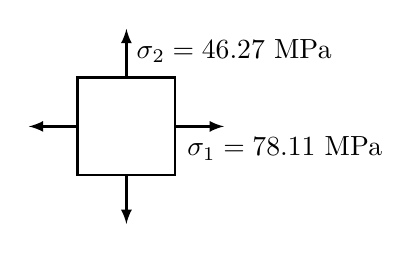
\begin{tikzpicture}[scale=0.62]
%square
\draw[thick] (-1,1) -- (1,1) -- (1,-1) -- (-1,-1) -- cycle;

%arrows
\draw[thick,-latex] (0,1) -- (0,2) node[below right] {$\sigma_2=46.27$ MPa};
\draw[thick,-latex] (1,0) -- (2,0)  node[below=8pt,right=-1.7em] {$\sigma_1=78.11$ MPa};
\draw[thick,-latex] (0,-1) -- (0,-2);
\draw[thick,-latex] (-1,0) -- (-2,0);
\end{tikzpicture}
\caption{2D principal stress element for pressure vessel.}
\label{fig:2dSquare}
\end{figure}

\begin{figure}[H]
\centering
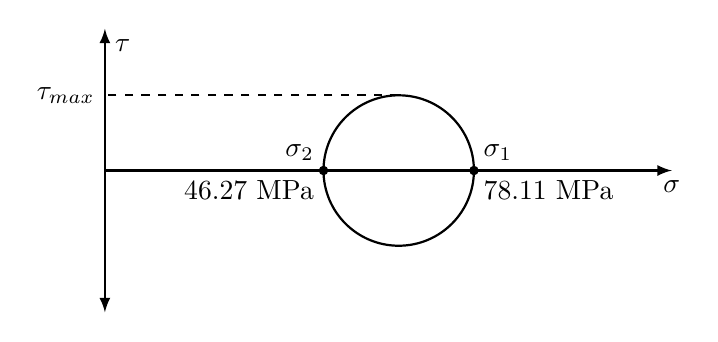
\begin{tikzpicture}[scale=0.6]
%axis
\draw[thick,latex-latex] (0,-3) -- (0,3) node[anchor=north west] {$\tau$};
\draw[thick,-latex] (0,0) -- (12,0) node[anchor=north] {$\sigma$};

%circle
\draw[thick] (6.219,0) circle (1.592);

%taumax
\draw[thick,dashed] (6.219,1.592) -- (0,1.592) node[left] {$\tau_{max}$};

%nodes
\filldraw[black] (4.627,0) circle (2.5pt);
\node[above left] at (4.627,0) {$\sigma_2$};
\node[below left] at (4.627,0) {46.27 MPa};
\filldraw[black] (7.811,0) circle (2.5pt);
\node[above right] at (7.811,0) {$\sigma_1$};
\node[below right] at (7.811,0) {78.11 MPa};
\end{tikzpicture}
\caption{Principal stresses plotted on Mohr’s circle diagram.}
\label{fig:Mohr}
\end{figure}

These principal stresses are comparable to the longitudinal and hoop stresses in the pressure vessel.
Theoretically, the ratio between hoop and longitudinal stress should be 2, so the relationship given by \eqref{eq:longStress} should hold for this pressure vessel.
However, this ratio is found to be 1.68 experimentally.
This may be in part because the strain gauges are used to measure compressive rather than tensile strains when opening the can.
The \ang{90} strain gauge sees less change than the \ang{0} strain gauge does, so the change in $\varepsilon_x$ is more difficult to record.
There may also be losses due to the adhesive used to affix the strain gauges to the can, as this may affect the strain measured in the aluminum.

\begin{table}[H]
\renewcommand\arraystretch{1.25}
\centering
\caption{Calculated Stresses and Strains}
\begin{tabular}{cc}
\hline \hline
Property & Value \\
\hline
$\varepsilon_x$ & 0.000873 $\pm$ 0.000014 mm/mm \\
$\varepsilon_\theta$ & 0.000828 $\pm$ 0.000010 mm/mm \\
$\varepsilon_y$ & 0.000299 $\pm$ 0.000005 mm/mm \\
$\gamma_{xy}$ & 0.000242 $\pm$ 0.000013 mm/mm \\
$\varepsilon_1$ & 0.000897 $\pm$ 0.000014 mm/mm \\
$\varepsilon_2$ & 0.000274 $\pm$ 0.000006 mm/mm \\
$\sigma_1$ & 78.11 $\pm$ 1.128 MPa \\
$\sigma_2$ & 46.27 $\pm$ 0.677 MPa \\
\hline \hline
\end{tabular}
\label{tab:CalcedStr}
\end{table}

\subsection{Pressure from Mechanics of Materials}

Three different pressure estimates are calculated under different assumptions about the calculated principal stress state.
The first pressure, $P_{\varepsilon_1}$, is calculated from the first principal strain, $\varepsilon_1$, by solving \eqref{eq:princStrainFin} for pressure and substituting one half the diameter, $d$, for radius, $r$.
\begin{equation}
\label{eq:Peps1}
P_{\varepsilon_1} = \frac{4Et\varepsilon_1}{d(2-\nu)}
\end{equation}

This pressure estimates that the associated principal stress state describes the hoop and longitudinal stresses of the pressure vessel.
By extension, this pressure estimate also assumes that $\sigma_1$ is double $\sigma_2$ despite this not being true for the associated principal stress state.

The second pressure, $P_{\sigma_1}$, is calculated from the first principal stress by solving \eqref{eq:hoopStress} for pressure and substituting one half the diameter, $d$, for radius, $r$.
\begin{equation}
\label{eq:Psig1}
P_{\sigma_1} = \frac{2t\sigma_1}{d}
\end{equation}
This pressure estimate assumes that the first principal stress, $\sigma_1$, is representative of the hoop stress $\sigma_H$.

The third pressure, $P_{\sigma_2}$, is calculated from the second principal stress by substituting \eqref{eq:longStress} into \eqref{eq:hoopStress}, solving for pressure, and substituting one half the diameter, $d$, for radius, $r$.
\begin{equation}
\label{eq:Psig2}
P_{\sigma_2} = \frac{4t\sigma_2}{d}
\end{equation}
This pressure estimate assumes that the second principal stress, $\sigma_2$, is representative of the longitudinal stress $\sigma_L$.

The decision on which of these three pressure estimates to use is dependent on the context in which it is used.
This report assumes that determining the pressure drop in a pressure vessel would be used in the design of a system to handle this pressure.
For this assumption, the highest estimated pressure, $P_{\sigma_2}$, is reported as the pressure drop estimate using the mechanics of materials method.

\begin{table}[H]
\renewcommand\arraystretch{1.25}
\centering
\caption{Calculated Pressures}
\begin{tabular}{cc}
\hline \hline
Property & Value (kPa) \\
\hline
$P_{\varepsilon_1}$ & 205 $\pm$ 35.3 \\
$P_{\sigma_1}$ & 213 $\pm$ 36.6 \\
$P_{\sigma_2}$ & 252 $\pm$ 43.4 \\
$P_{IGL}$ & 258 $\pm$ 57.2 \\
\hline \hline
\end{tabular}
\label{tab:CalcedP}
\end{table}

\subsection{Pressure from Ideal Gas Law}

The pressure calculated from the ideal gas law method is $P_{IGL}=258$ $\pm$ 57.15 kPa.
This secondary method was performed on a different beverage can than the mechanics of materials method can, so this was initially to be useful as an order of magnitude comparison rather than an exact validation.
However, the pressure result of the second method falls within 10 kPa of the mechanics of materials reported result, allowing for some level of confidence in the pressure results.

\subsection{Comparing Pressure Calculation Methods}

The uncertainty in the mechanics of materials method pressure is $\pm$43.4 kPa, and the uncertainty in the ideal gas method is $\pm$57.2 kPa, 14 kPa more than the uncertainty in the mechanics of materials method.
This may indicate that the mechanics of materials method is more effective than the ideal gas method in determining can pressure.
However, these values are near enough to one another that either method could be used to determine can pressure with comparable reliability.

\subsection{Comparison Across Course-wide Data Set}

The mean pressure excluding outliers across all lab groups in the Spring 2022 section is 261.32 kPa, with a standard deviation of 86.04 kPa.
The calculated pressure for the selected data set is within 10 kPa of this mean value, and well within the standard deviation.
The standard deviation is rather large, almost a third of the mean value, so this does not necessarily communicate accuracy, but this does indicate that the computed pressures above are within the proper order of magnitude for the other beverage cans.
The mean pressure value for Dr. Pepper is 256.1 kPa and the mean value for Pepsi is 260.8 kPa, but with standard deviations of 88.9 kPa and 57.7 kPa respectively, it is difficult to say with confidence the type of beverage used in the selected data set.

\section{Conclusion}

This study uses the principles of mechanics of materials to determine the pressure in an unopened soda can treated as a thin-walled pressure vessel.
Thin-walled pressure vessel theory applied to principal stress theory allows an experimenter to calculate the internal pressure.
This result is compared to a secondary method based upon the ideal gas law.
The hoop stress in the can is 78.11 $\pm$ 1.128 MPa and the longitudinal stress is 46.27 $\pm$ 0.677 MPa.
The internal pressure reported by the mechanics of materials approach is 252 $\pm$ 43.4 kPa. The internal pressure reported by the ideal gas law method is 258 $\pm$ 57.2 kPa.

\section*{Appendix A: Uncertainty Calculation}

The uncertainty of each variable is given by Table \ref{tab:Uncertainty}.
The uncertainties in $V_{amp_{x}}$, $V_{amp_{\theta}}$, $V_{amp_{y}}$, and $V_{s}$ were calculated by finding the standard deviation of a large sample set of these measurements and approximating a 95\% confidence interval.
The uncertainties in $d$ and $t$ were determined from the measuring device used, which was a micrometer.
The uncertainties in the weights of the can and the water were determined from the scale that was used.
The uncertainties in $E$, $\nu$, $R$, $M$, and $\rho$ were estimated to be $\pm$1\% of the given value due to variability associated with these material properties.
\begin{table}[H]
\renewcommand\arraystretch{1.25}
\centering
\caption{Uncertainty in Each Variable}
\resizebox{3.5in}{!}{\begin{tabular}{ccc}
\hline \hline
Variable (Symbol) & Value & Uncertainty \\
\hline
Initial Amplified Voltage $x$ ($V_{amp_{xi}}$) & $-$0.1389 V & $\pm$0.00056 V \\
Initial Amplified Voltage $\theta$ ($V_{amp_{\theta i}}$) & 0.0674 V & $\pm$0.00039 V \\
Initial Amplified Voltage $y$ ($V_{amp_{yi}}$) & $-$0.1064 V & $\pm$0.00052 V \\
Final Amplified Voltage $x$ ($V_{amp_{xf}}$) & $-$0.2367 V & $\pm$0.0011 V \\
Final Amplified Voltage $\theta$ ($V_{amp_{\theta f}}$) & $-$0.0253 V & $\pm$0.00027 V \\
Final Amplified Voltage $y$ ($V_{amp_{yf}}$) & $-$0.1398 V & $\pm$0.00055 V \\
Excitation Voltage ($V_s$) & 3.349 V &  $\pm$0.002 V \\
Can Diameter ($d$) & 66.63 mm & $\pm$0.89 mm \\
Can Thickness ($t$) & 0.091 mm & $\pm$0.016 mm \\
Modulus of Elasticity ($E$) \cite{b3} & 69 GPa & $\pm$0.69 GPa \\
Poisson's Ratio ($\nu$) \cite{b3} & 0.35 & $\pm$0.0035 \\
%Shear Modulus ($G$) \cite{b3} & 25 GPa & $\pm$0.25 GPa \\
Gauge Factor ($G_f$) & 2.09 & $\pm$0.01045 \\
Gain ($A$) & 64 & $\pm$0.64 \\
Initial Can Weight ($W_{ci}$) & 406.8 g & $\pm$0.1 g \\
Final Can Weight ($W_{cf}$) & 406.2 g & $\pm$0.1 g \\
Initial Water Weight ($W_{wi}$) & 152.0 g & $\pm$0.1 g \\
Final Water Weight ($W_{wf}$) & 141.4 g & $\pm$0.1 g \\
Temperature ($T$) & 22.78$^\circ$C & $\pm$0.28$^\circ$C \\
Gas Constant ($R$) \cite{b6} & 8.31 \unit{\joule\per\kelvin\per\mole} & $\pm$0.083 \unit{\joule\per\kelvin\per\mole} \\
CO\textsubscript{2} Molar Mass ($M$) \cite{b4} & 44 \unit{\gram\per\mole} & $\pm$0.44 \unit{\gram\per\mole} \\
Density of Water ($\rho$) \cite{b7} & 0.998 \unit{\gram\per\centi\meter\cubed} & $\pm$0.00998 \unit{\gram\per\centi\meter\cubed} \\
\hline \hline
\end{tabular}}
\label{tab:Uncertainty}
\end{table}

\subsection*{Uncertainty in $\Delta V_{amp}$}

The change in $V_{amp}$ for each strain gauge can be calculated using \eqref{eq:deltaVamp}, where $V_{amp_{xi}}$, $V_{amp_{\theta i}}$, and $V_{amp_{yi}}$ are the initial voltages and $V_{amp_{xf}}$, $V_{amp_{\theta f}}$, and $V_{amp_{yf}}$ are the final voltages.
\begin{subequations}
\label{eq:deltaVamp}
\begin{align}
\Delta V_{amp_{x}}&=V_{amp_{xf}}-V_{amp_{xi}} \\
\Delta V_{amp_{\theta}}&=V_{amp_{\theta f}}-V_{amp_{\theta i}} \\
\Delta V_{amp_{y}}&=V_{amp_{yf}}-V_{amp_{yi}}
\end{align}
\end{subequations}
The uncertainty in each $\Delta V_{amp}$ can be calculated using the root sum square (RSS) method and \eqref{eq:deltaVamp}, where $U$ is the uncertainty.
\begin{equation}
\label{eq:UDeltaVamp}
\resizebox{227pt}{!}{$U_{\Delta V_{amp}}=\left[U_{V_{amp_{i}}}^2 \left(\frac{\partial (\Delta V_{amp})}{\partial V_{amp_{i}}}\right)^2 + U_{V_{amp_{f}}}^2 \left(\frac{\partial (\Delta V_{amp})}{\partial V_{amp_{f}}}\right)^2 \right]^{\frac{1}{2}}$}
\end{equation}
For $V_{amp_{x}}$, using the values given in Table \ref{tab:Uncertainty} give an uncertainty in $\Delta V_{amp_{x}}$ of $\pm$0.27 V.

\subsection*{Uncertainty in Strain}

Strain is given by \eqref{eq:strain}.
The uncertainty in strain can be calculated by using \eqref{eq:UStrain}.
\begin{equation}
\label{eq:UStrain}
\resizebox{227pt}{!}{$U_{\varepsilon}=\left[U_{\Delta V_{amp}}^2 \left(\frac{\partial \varepsilon}{\partial (\Delta V_{amp})}\right)^2 + U_{A}^2 \left(\frac{\partial \varepsilon}{\partial A}\right)^2 + U_{V_s}^2 \left(\frac{\partial \varepsilon}{\partial V_s}\right)^2 + U_{G_f}^2 \left(\frac{\partial \varepsilon}{\partial G_f}\right)^2 \right]^{\frac{1}{2}}$}
\end{equation}
For $\Delta V_{amp_{x}}$, using the values given in Table \ref{tab:Uncertainty} give an uncertainty in strain $\varepsilon_x$ of $\pm$0.000014 mm/mm.

\subsection*{Uncertainty in Shear Strain}

Shear strain for a 0-45-\ang{90} rosette is given by \eqref{eq:shearStr}.
\begin{equation}
\label{eq:shearStr}
\gamma_{xy}=\varepsilon_\theta - \frac{\varepsilon_x+\varepsilon_y}{2}
\end{equation}
The uncertainty in shear strain can be calculated by using \eqref{eq:UShearStrain}.
\begin{equation}
\label{eq:UShearStrain}
U_{\gamma_{xy}}=\left[U_{\varepsilon_x}^2 \left(\frac{\partial \gamma_{xy}}{\partial \varepsilon_x}\right)^2 + U_{\varepsilon_\theta}^2 \left(\frac{\partial \gamma_{xy}}{\partial \varepsilon_\theta}\right)^2 + U_{\varepsilon_y}^2 \left(\frac{\partial \gamma_{xy}}{\partial \varepsilon_y}\right)^2 \right]^{\frac{1}{2}}
\end{equation}
Using Table \ref{tab:CalcedStr}, the uncertainty in shear strain is $\pm$0.000013 mm/mm.

\subsection*{Uncertainty in Principle Strain}

Principle strain is given by \eqref{eq:princStrain}.
The uncertainty in principle strain can be calculated by using \eqref{eq:UPrincStrain}.
\begin{equation}
\label{eq:UPrincStrain}
\resizebox{227pt}{!}{$U_{\varepsilon_{1,2}}=\left[U_{\varepsilon_x}^2 \left(\frac{\partial \varepsilon_{1,2}}{\partial \varepsilon_x}\right)^2 + U_{\varepsilon_y}^2 \left(\frac{\partial \varepsilon_{1,2}}{\partial \varepsilon_y}\right)^2 + U_{\gamma_{xy}}^2 \left(\frac{\partial \varepsilon_{1,2}}{\partial \gamma_{xy}}\right)^2 \right]^{\frac{1}{2}}$}
\end{equation}
For $\varepsilon_1$, using Table \ref{tab:CalcedStr} gives an uncertainty in principle strain $\varepsilon_1$ of $\pm$0.000014 mm/mm.

\subsection*{Uncertainty in Principle Stress}

Principle stress is given by \eqref{eq:sigmas}.
The uncertainty in principle stress can be calculated by using \eqref{eq:UPrincStress}.
\begin{equation}
\label{eq:UPrincStress}
\resizebox{227pt}{!}{$U_{\sigma_{1,2}}=\left[U_{E}^2 \left(\frac{\partial \sigma_{1,2}}{\partial E}\right)^2 + U_{\nu}^2 \left(\frac{\partial \sigma_{1,2}}{\partial \nu}\right)^2 + U_{\varepsilon_1}^2 \left(\frac{\partial \sigma_{1,2}}{\partial \varepsilon_1}\right)^2 + U_{\varepsilon_2}^2 \left(\frac{\partial \sigma_{1,2}}{\partial \varepsilon_2}\right)^2 \right]^{\frac{1}{2}}$}
\end{equation}
For $\sigma_1$, using Table \ref{tab:CalcedStr} and the values given in Table \ref{tab:Uncertainty} gives an uncertainty in principle stress $\sigma_1$ of $\pm$0.677 MPa.

\subsection*{Uncertainty in Pressure from Stress}

Pressure from stress is given by \eqref{eq:Psig1} and \eqref{eq:Psig2}.
The uncertainty in pressure can be calculated by using \eqref{eq:UPressStrain}.
\begin{equation}
\label{eq:UPressStrain}
U_{P}=\left[U_{\sigma_{1,2}}^2 \left(\frac{\partial P}{\partial \sigma_{1,2}}\right)^2 + U_{t}^2 \left(\frac{\partial P}{\partial t}\right)^2 + U_{d}^2 \left(\frac{\partial P}{\partial d}\right)^2 \right]^{\frac{1}{2}}
\end{equation}
For $\sigma_1$, using Table \ref{tab:MoMProp}, Table \ref{tab:CalcedStr}, and the values given in Table \ref{tab:Uncertainty} gives an uncertainty in pressure from stress $P_{\sigma_1}$ of $\pm$36.6 kPa.

\subsection*{Uncertainty in Amount of Substance}

The amount of substance $n$ is given by \eqref{eq:moles}.
The uncertainty in the amount of substance can be calculated by using \eqref{eq:Uamt}.
\begin{equation}
\label{eq:Uamt}
\resizebox{227pt}{!}{$U_{n}=\left[U_{W_{ci}}^2 \left(\frac{\partial n}{\partial W_{ci}}\right)^2 + U_{W_{cf}}^2 \left(\frac{\partial n}{\partial W_{cf}}\right)^2 + U_{M}^2 \left(\frac{\partial n}{\partial M}\right)^2 \right]^{\frac{1}{2}}$}
\end{equation}
Using Table \ref{tab:IGLProp} and the values given in Table \ref{tab:Uncertainty} gives an uncertainty in the amount of substance of $\pm$0.0032 mol.

\subsection*{Uncertainty in Volume}

Volume is given by \eqref{eq:vol}.
The uncertainty in volume can be calculated by using \eqref{eq:Uvol}.
\begin{equation}
\label{eq:Uvol}
\resizebox{227pt}{!}{$U_{V}=\left[U_{W_{wi}}^2 \left(\frac{\partial V}{\partial W_{wi}}\right)^2 + U_{W_{wf}}^2 \left(\frac{\partial V}{\partial W_{wf}}\right)^2 + U_{\rho}^2 \left(\frac{\partial V}{\partial \rho}\right)^2 \right]^{\frac{1}{2}}$}
\end{equation}
Using Table \ref{tab:IGLProp} and the values given in Table \ref{tab:Uncertainty} gives an uncertainty in volume of $\pm$0.178 \unit{\centi\meter\cubed}.

\subsection*{Uncertainty in Pressure from Ideal Gas Law}

Pressure from the ideal gas law is given by \eqref{eq:PIGL}.
The uncertainty in pressure can be calculated by using \eqref{eq:UPressIGL}.
\begin{equation}
\label{eq:UPressIGL}
\resizebox{227pt}{!}{$U_{P_{IGL}}=\left[U_{n}^2 \left(\frac{\partial P_{IGL}}{\partial n}\right)^2 + U_{R}^2 \left(\frac{\partial P_{IGL}}{\partial R}\right)^2 + U_{T}^2 \left(\frac{\partial P_{IGL}}{\partial T}\right)^2 + U_{V}^2 \left(\frac{\partial P_{IGL}}{\partial V}\right)^2 \right]^{\frac{1}{2}}$}
\end{equation}
Using the values given in Table \ref{tab:Uncertainty}, and the uncertainties calculated in the previous sections gives an uncertainty in pressure from the ideal gas law of $\pm$57.2 kPa.

%\hfill\break
%\noindent
%This lab report was produced using \LaTeX.

\section*{Acknowledgment}

The authors would like to thank Dr. Ridgeway and the Fall 2021 lab group for supplying data for analysis.

\begin{thebibliography}{00}
\bibitem{b1} G. Subhash and S. Ridgeway, ``Thin-walled Pressure Vessels," in \textit{Mechanics of Materials Laboratory Course}. San Rafael, CA: Morgan \& Claypool, 2018, ch. 3, pp. 113--132.
\bibitem{b5} S. Ridgeway. (2022). Lab 3 Discussion, Final Project Track 1 [PowerPoint slides]. Available: \url{https://ufl.instructure.com/courses/447927/files/67779901}
\bibitem{b2} D. R. Askeland, F. Haddleton, P. Green, and H. Robertson, ``Nonferrous Alloys," in \textit{The Science and Engineering of Materials}, 3rd ed. Berlin, Germany: Springer, 1996, ch. 13, pp. 401--436.
\bibitem{b9} H. de Grys, ``Determining the pressure inside an unopened carbonated beverage," \textit{Journal of Chemical Education}, vol. 84, no. 7, pp. 1117--1119, Jul. 2007. [Online]. Available: \url{https://doi.org/10.1021/ed084p1117}
\bibitem{b10} S. Ridgeway. (2022). Final Project [PowerPoint slides]. Available: \url{https://ufl.instructure.com/courses/447927/files/67906146}
\bibitem{b3} J. W. Bray, ``Aluminum Mill and Engineered Wrought Products," in \textit{Properties and Selection: Nonferrous Alloys and Special-Purpose Materials} (ASM Handbook, Vol. 2). Russell Township, OH: ASM International, 1990.
\bibitem{b6} Engineering ToolBox. (2004). \textit{Universal and Individual Gas Constants}. [Online] Available: \url{https://www.engineeringtoolbox.com/individual-universal-gas-constant-d_588.html}
\bibitem{b4} Engineering ToolBox. (2018). \textit{Carbon Dioxide - Thermophysical Properties}. [Online] Available: \url{https://www.engineeringtoolbox.com/CO2-carbon-dioxide-properties-d_2017.html}
\bibitem{b7} Engineering ToolBox. (2003). \textit{Water - Density, Specific Weight and Thermal Expansion Coefficients}. [Online] Available: \url{https://www.engineeringtoolbox.com/water-density-specific-weight-d_595.html}
%\bibitem{b8} S. Ridgeway. (2022). Lab 2 Report, Uncertainty [PowerPoint slides]. Available: \url{https://ufl.instructure.com/courses/447927/files/66505329}
\end{thebibliography}

\end{document}
